\documentclass[12pt, titlepage]{article}

\usepackage{booktabs}
\usepackage{graphicx}
\usepackage{tabularx}
\usepackage{hyperref}
\hypersetup{
    colorlinks,
    citecolor=black,
    filecolor=black,
    linkcolor=red,
    urlcolor=blue
}
\usepackage[round]{natbib}

\usepackage{longtable}

%% Comments

\usepackage{color}

\newif\ifcomments\commentstrue %displays comments
%\newif\ifcomments\commentsfalse %so that comments do not display

\ifcomments
\newcommand{\authornote}[3]{\textcolor{#1}{[#3 ---#2]}}
\newcommand{\todo}[1]{\textcolor{red}{[TODO: #1]}}
\else
\newcommand{\authornote}[3]{}
\newcommand{\todo}[1]{}
\fi

\newcommand{\wss}[1]{\authornote{blue}{SS}{#1}} 
\newcommand{\plt}[1]{\authornote{magenta}{TPLT}{#1}} %For explanation of the template
\newcommand{\an}[1]{\authornote{cyan}{Author}{#1}}
%% Common Parts

\newcommand{\progname}{Software Engineering} % PUT YOUR PROGRAM NAME HERE
\newcommand{\authname}{Team \#12, Lower Earth Orbiters
\\ Diamond Ahuja
\\ Rishi Vaya
\\ Buu Ha
\\ Dhruv Cheemakurti
\\ Umang Rajkarnikar} % AUTHOR NAMES                  

\usepackage{hyperref}
    \hypersetup{colorlinks=true, linkcolor=blue, citecolor=blue, filecolor=blue,
                urlcolor=blue, unicode=false}
    \urlstyle{same}
                                


\begin{document}

\title{Verification and Validation Report: \progname} 
\author{\authname}
\date{\today}
	
\maketitle

\pagenumbering{roman}

\section{Revision History}

\begin{tabularx}{\textwidth}{p{3cm}p{2cm}X}
\toprule {\bf Date} & {\bf Version} & {\bf Notes}\\
\midrule
March 6, 2024 & 1.0 & Upload VnVReport - U.R.\\
April 2, 2024 & 2.0 & Update VnVReport with feedback - U.R.\\
April 3, 2024 & 2.1 & Label tables and better organize information - U.R.\\
April 3, 2024 & 2.2 & Updated traceability matrices - U.R.\\
\bottomrule
\end{tabularx}

~\newpage

\section{Symbols, Abbreviations and Acronyms}

\renewcommand{\arraystretch}{1.2}
\begin{tabular}{l l} 
  \toprule		
  \textbf{symbol} & \textbf{description}\\
  \midrule 
  ObjectID & MongoDB Record/Document Id\\
  DB & Database\\
  Schedule & Model type for MongoDB Schedule Collection \\
  Command & Model type for MongoDB Command Collection \\
  VM & Virtual Machine \\
  NEUDOSE & NEUtron DOSimetry Exploration \\
  UI/UX & User Interface/User Experience \\
  JSON & JavaScript Object Notation \\
  \bottomrule
\end{tabular}\\

\newpage

\tableofcontents

\listoftables %if appropriate

\listoffigures %if appropriate

\newpage

\pagenumbering{arabic}

\section{Functional Requirements Evaluation}

\subsection{MCT Application Accessibility}

\begin{center}
\begin{longtable}{|p{2cm} | p{8cm} |p{2cm}| }
\caption{MCT Application Accessibility Tests}
\hline
\textbf{Test Id} & \textbf{Notes} & \textbf{Result} \\
\hline
FR-SLN1 & MCT application is a site hosted on Netlify which was accessed manually using Safari, Chrome and Firefox & Pass \\
\hline
FR-SLN2 & Manually established a connection on a TCP port and sent linux-commands through this port & Pass \\
\hline

\end{longtable}
\end{center}

\subsection{Managing User Roles}

\begin{center}
\begin{longtable}{|p{2cm} | p{8cm} |p{2cm}| }
\caption{Managing User Roles Tests}
\hline
\textbf{Test Id} & \textbf{Notes} & \textbf{Result} \\
\hline
FR-SLN3 & Manually created a new user through the MCT's frontend facing application & Pass \\
\hline
FR-SLN4 & Manually edited and removed a user through the MCT's frontend facing application & Pass \\
\hline

\end{longtable}
\end{center}

\subsection{Scheduling and Executing Commands}

\begin{center}
\begin{longtable}{|p{2cm} | p{8cm} |p{2cm}| }
\caption{Scheduling and Executing Commands Tests}
\hline
\textbf{Test Id} & \textbf{Notes} & \textbf{Result} \\
\hline
FR-SLN5 & The addition, modification, and deletion of command sequences have been tested manually through the frontend. & Pass \\
\hline
FR-SLN6 & Manually executed a scheduled command sequence and viewed output through the frontend. & Pass \\
\hline

\end{longtable}
\end{center}

\subsection{Cancelling Commands}

\begin{center}
\begin{longtable}{|p{2cm} | p{8cm} |p{2cm}| }
\caption{Cancelling Commands Tests}
\hline
\textbf{Test Id} & \textbf{Notes} & \textbf{Result} \\
\hline
FR-SLN7 & The cancellation of command sequences have been tested manually through the frontend. & Pass \\
\hline

\end{longtable}
\end{center}

\subsection{Validating Scheduled Commands}

\begin{center}
\begin{longtable}{|p{2cm} | p{8cm} |p{2cm}| }
\caption{Validating Scheduled Commands Tests}
\hline
\textbf{Test Id} & \textbf{Notes} & \textbf{Result} \\
\hline
FR-SLN8 & Manually tested through the frontend. & Pass \\
\hline

\end{longtable}
\end{center}

\subsection{Permission List Criteria for User}

\begin{center}
\begin{longtable}{|p{2cm} | p{8cm} |p{2cm}| }
\caption{Permission List Criteria for User Tests}
\hline
\textbf{Test Id} & \textbf{Notes} & \textbf{Result} \\
\hline
FR-SLN9 & Manually tested execution of invalid command sequence through the frontend. & Pass \\
\hline

\end{longtable}
\end{center}

\subsection{Permission List Criteria for Command Target}

\begin{center}
\begin{longtable}{|p{2cm} | p{8cm} |p{2cm}| }
\caption{Permission List Criteria for Command Target Tests}
\hline
\textbf{Test Id} & \textbf{Notes} & \textbf{Result} \\
\hline
FR-SLN11 & Manually tested execution of invalid command sequence through the frontend. & Pass \\
\hline

\end{longtable}
\end{center}

\subsection{Managing Scheduled Command Sequences}

\begin{center}
\begin{longtable}{|p{2cm} | p{8cm} |p{2cm}| }
\caption{Managing Scheduled Command Sequences Tests}
\hline
\textbf{Test Id} & \textbf{Notes} & \textbf{Result} \\
\hline
FR-SLN12 & Manually tested managing (adding, deleting, editing) list of command sequences. & Pass \\
\hline

\end{longtable}
\end{center}

\subsection{Selecting and Editing Satellites}

\begin{center}
\begin{longtable}{|p{2cm} | p{8cm} |p{2cm}| }
\caption{Selecting and Editing Satellites Tests}
\hline
\textbf{Test Id} & \textbf{Notes} & \textbf{Result} \\
\hline
FR-SLN13 & Manually tested managing (adding, removing) satellites of interest through the frontend. & Pass \\
\hline

\end{longtable}
\end{center}

\subsection{Viewing Configured Satellites}

\begin{center}
\begin{longtable}{|p{2cm} | p{8cm} |p{2cm}| }
\caption{Viewing Configured Satellites Tests}
\hline
\textbf{Test Id} & \textbf{Notes} & \textbf{Result} \\
\hline
FR-SLN14 & Manually tested through the frontend. & Pass \\
\hline

\end{longtable}
\end{center}

New changes to FR-SLN14 have been made to test the fetching of the
data from external libraries (instead of testing for correctness). These
tests includes fetching the data based on the state of the TLE passed
in, Valid TLE, Invalid TLE, Valid Start Date, Invalid State Date, and
a combination of both.

\subsection{Detecting Satellite and Scheduling Command}

\begin{center}
\begin{longtable}{|p{2cm} | p{8cm} |p{2cm}| }
\caption{Detecting Satellite and Scheduling Command Tests}
\hline
\textbf{Test Id} & \textbf{Notes} & \textbf{Result} \\
\hline
FR-SLN16 & Unit tests hav been written to only executed on the date and time range specified for an overpass date. & Pass \\
\hline

\end{longtable}
\end{center}

\section{Nonfunctional Requirements Evaluation}

\subsection{Usability}

\begin{center}
\begin{longtable}{|p{4cm} | p{4cm}| }
\caption{Nonfunctional Requirements Evaluation Tests}
\hline
\textbf{Test Id} & \textbf{Result} \\
\hline
usability-1 & Pass \\
\hline
usability-2 & Pass \\
\hline

\end{longtable}
\end{center}
The tests above were conducted in two separate usability testing demonstrations, involving members from NEUDOSE's MIST team. All users involved in testing had no prior experience with the application, which focuses on their ability to learn and navigate the system independently. Both usability-1 and usability-2 had surveys to collect feedback for enhancement in the application’s design and functionality.
\\ \\
The feedback that we received from usability-1 the second
usability test, usability-2, which helped assess the application's usability.
\\ \\ 
Overall, users found the application intuitive to use while pointing out some areas for improvement. The data for this survey is attached below in Section ADD. In our first usability demonstration, we received a score of 3/5. Then after re-iterating our frontend design, we received a usability score of 5/5 from our stakeholders. This score measures how intuitive and easy it was for new users to identify core functionalities in the web application. Additionally, from usability-2 we found that it takes users on average less than five minutes to identify and explore the core use cases of the application.

usability-3 - NFR 10.5
\begin{itemize}
    \item After careful consideration, our team has decided not to proceed with the implementation of the accessibility-focused verification and validation (VnV) plan, as outlined under the Usability-3 category, NFR: 10.5. This decision reflects our current prioritization of resources and development efforts. 
    \item While we recognize the importance of accessibility in software development, our decision to forego this specific aspect of testing at this time allows us to allocate our resources towards other critical areas of development. We remain committed to creating an inclusive and accessible application and plan to revisit and incorporate comprehensive accessibility features and testing in future development phases. 
\end{itemize}
\subsection{Performance}

\begin{center}
\begin{longtable}{|p{4cm} | p{4cm}| }
\caption{Performance Tests}
\hline
\textbf{Test Id} & \textbf{Result} \\
\hline
performance-2 & Pass \\
\hline
performance-4 & Pass \\
\hline

\end{longtable}
\end{center}

For performance-2, we have deployed our application using external cloud providers. We use Netlify to host our frontend facing application and a DigitalOcean virtual machine to host our backend and server-side logic. In addition, we rely on the monitoring tools offered by these external providers to check the system's availablity and usage at regular intervals. The figures provided below illustrate the application's bandwidth, and CPU usage in the last hour. This time frame can also be specified for a longer duration. From the images below, our application is not very resource intensive where CPU usage is less than 1\%. The continuous monitoring tools configured on both DigitalOcean and Netlify provides notifications on the application's uptime and downtime. Since the deployment of the application, the system's overall uptime has been 100\% excluding scheduled maintenance periods. This is consistent with the availability that these cloud poviders offer, where both DigitalOcean and Netlify guarantees an uptime of 99.99\% for deployments.

\begin{figure}[h]
\centering
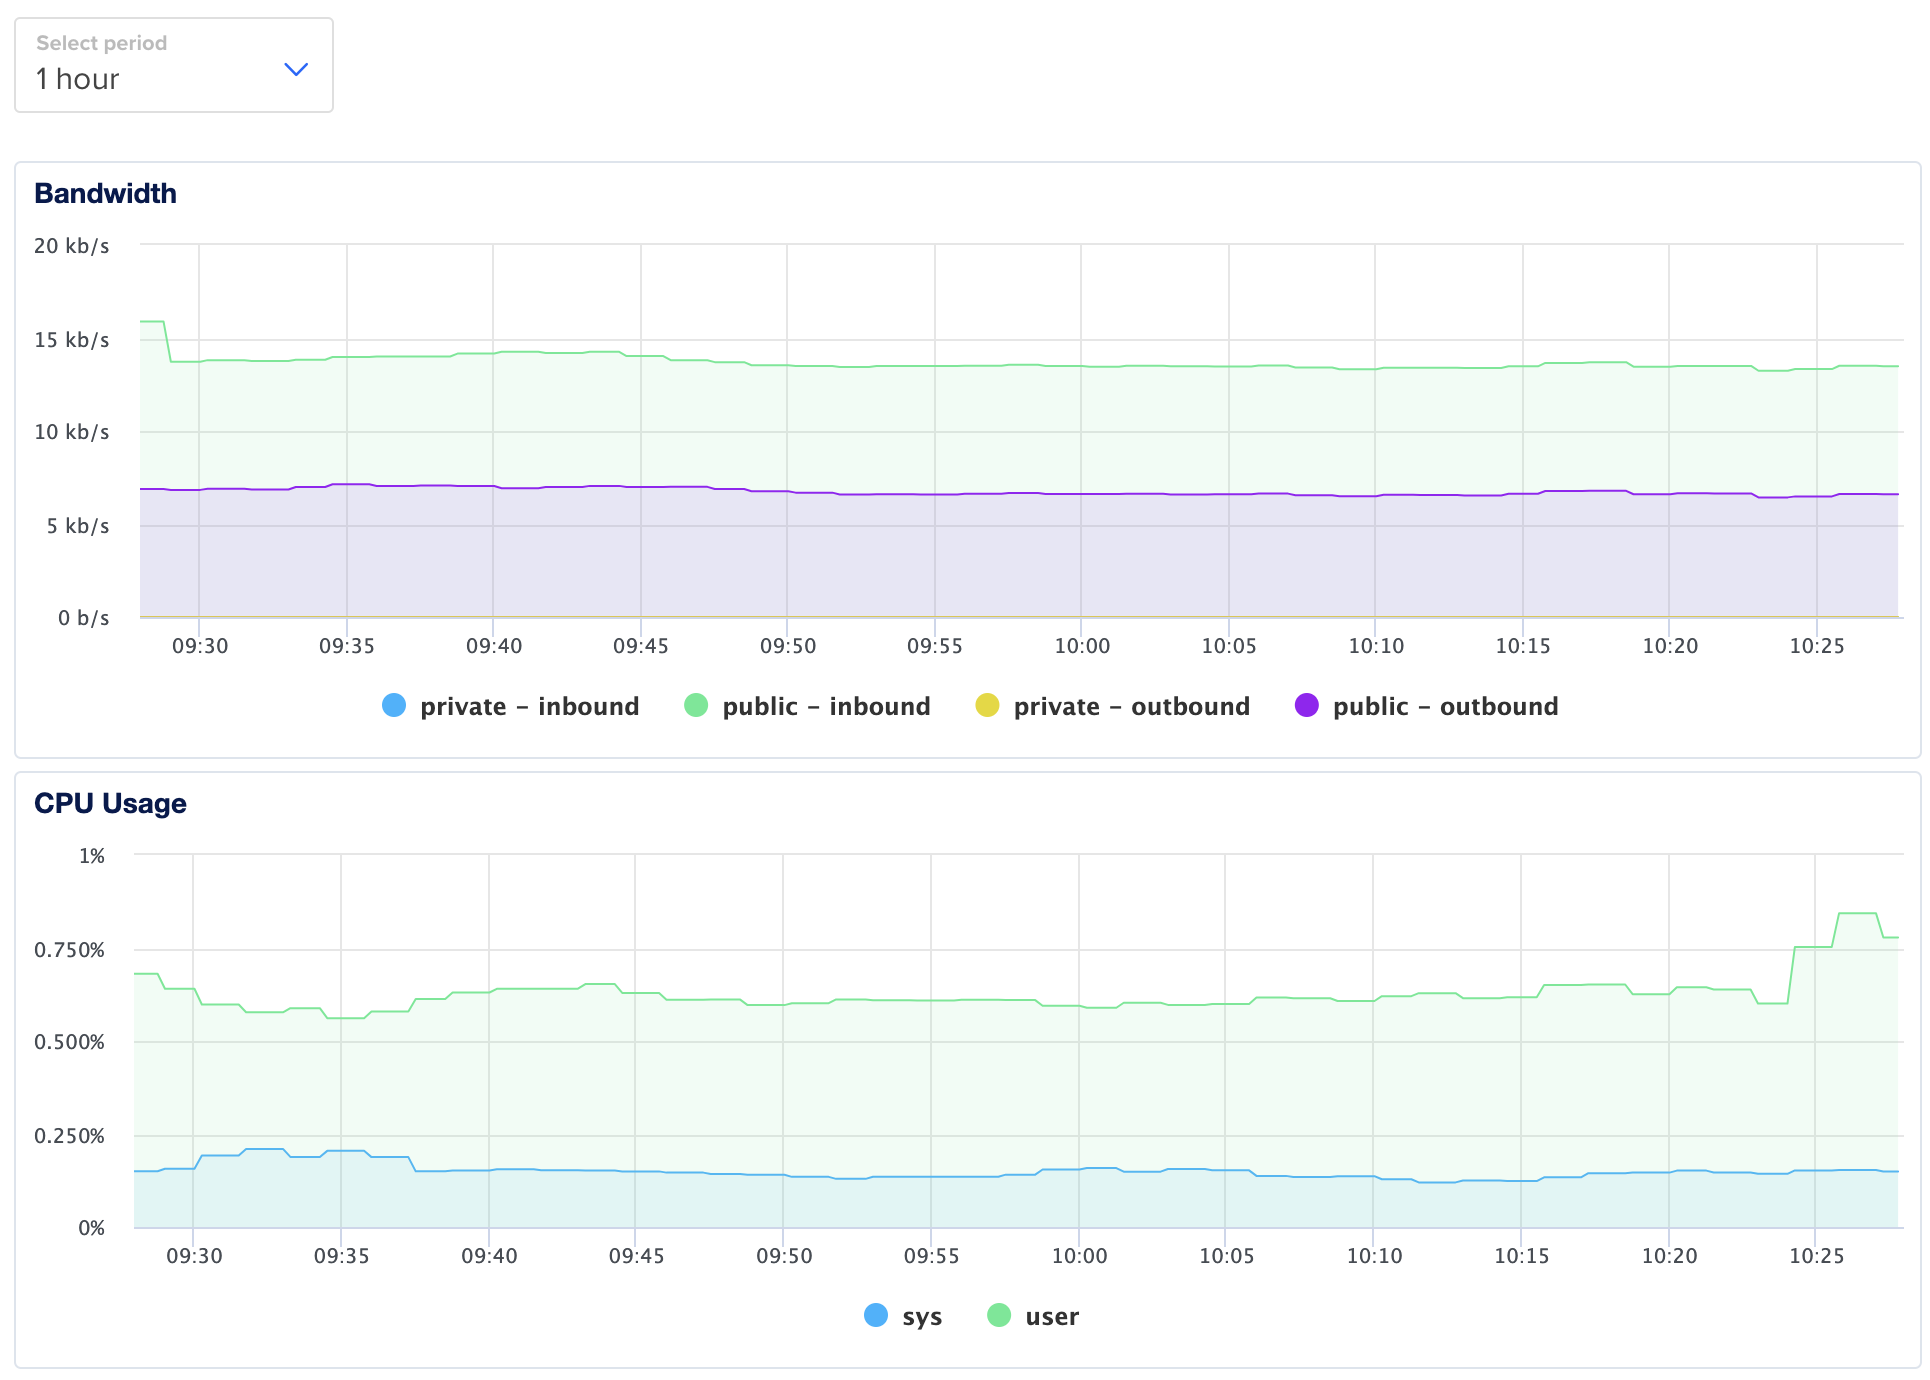
\includegraphics[width=1\textwidth]{performance-metrics.png}
\caption{Application usage in last hour}
\label{fig:myimage}
\end{figure}

\newpage

For performance-4, scenarios which cause internal exceptions have been identified and implemented in automatic test cases. These automated tests have been implemented using Jest.js. Several of these tests involve handling edge cases which aim to catch internal exceptions. The figure below showcases the results from running all 88 unit tests pertaining to the functionality of the Satellite, Schedule, Command, and User modules.


\begin{figure}[h]

\graphicspath{./jestResults/}
\includegraphics[width=15cm, height=10cm]{jestResults.png}
\caption{Jest.js Unit Test Results}
\end{figure}

\newpage


\subsection{Environmental}

\begin{center}
\begin{longtable}{|p{4cm} | p{4cm}| }
\caption{Environmental Tests}
\hline
\textbf{Test Id} & \textbf{Result} \\
\hline
environment-1 & Pass \\
\hline
environment-2 & Pass \\
\hline
environment-3 & Pass \\
\hline

\end{longtable}
\end{center}

For environmental-1, the application is setup to be hosted on Netlify's free service at the current moment. This applies that the features are also limited and that there cannot be a lot of traffic sent which makes testing the load much challenging. However, JMeter was used to verify the capabilities and challenged the application with 20 virtual users for 20 mintutes. Here are the results:

\begin{figure}[h]
\centering
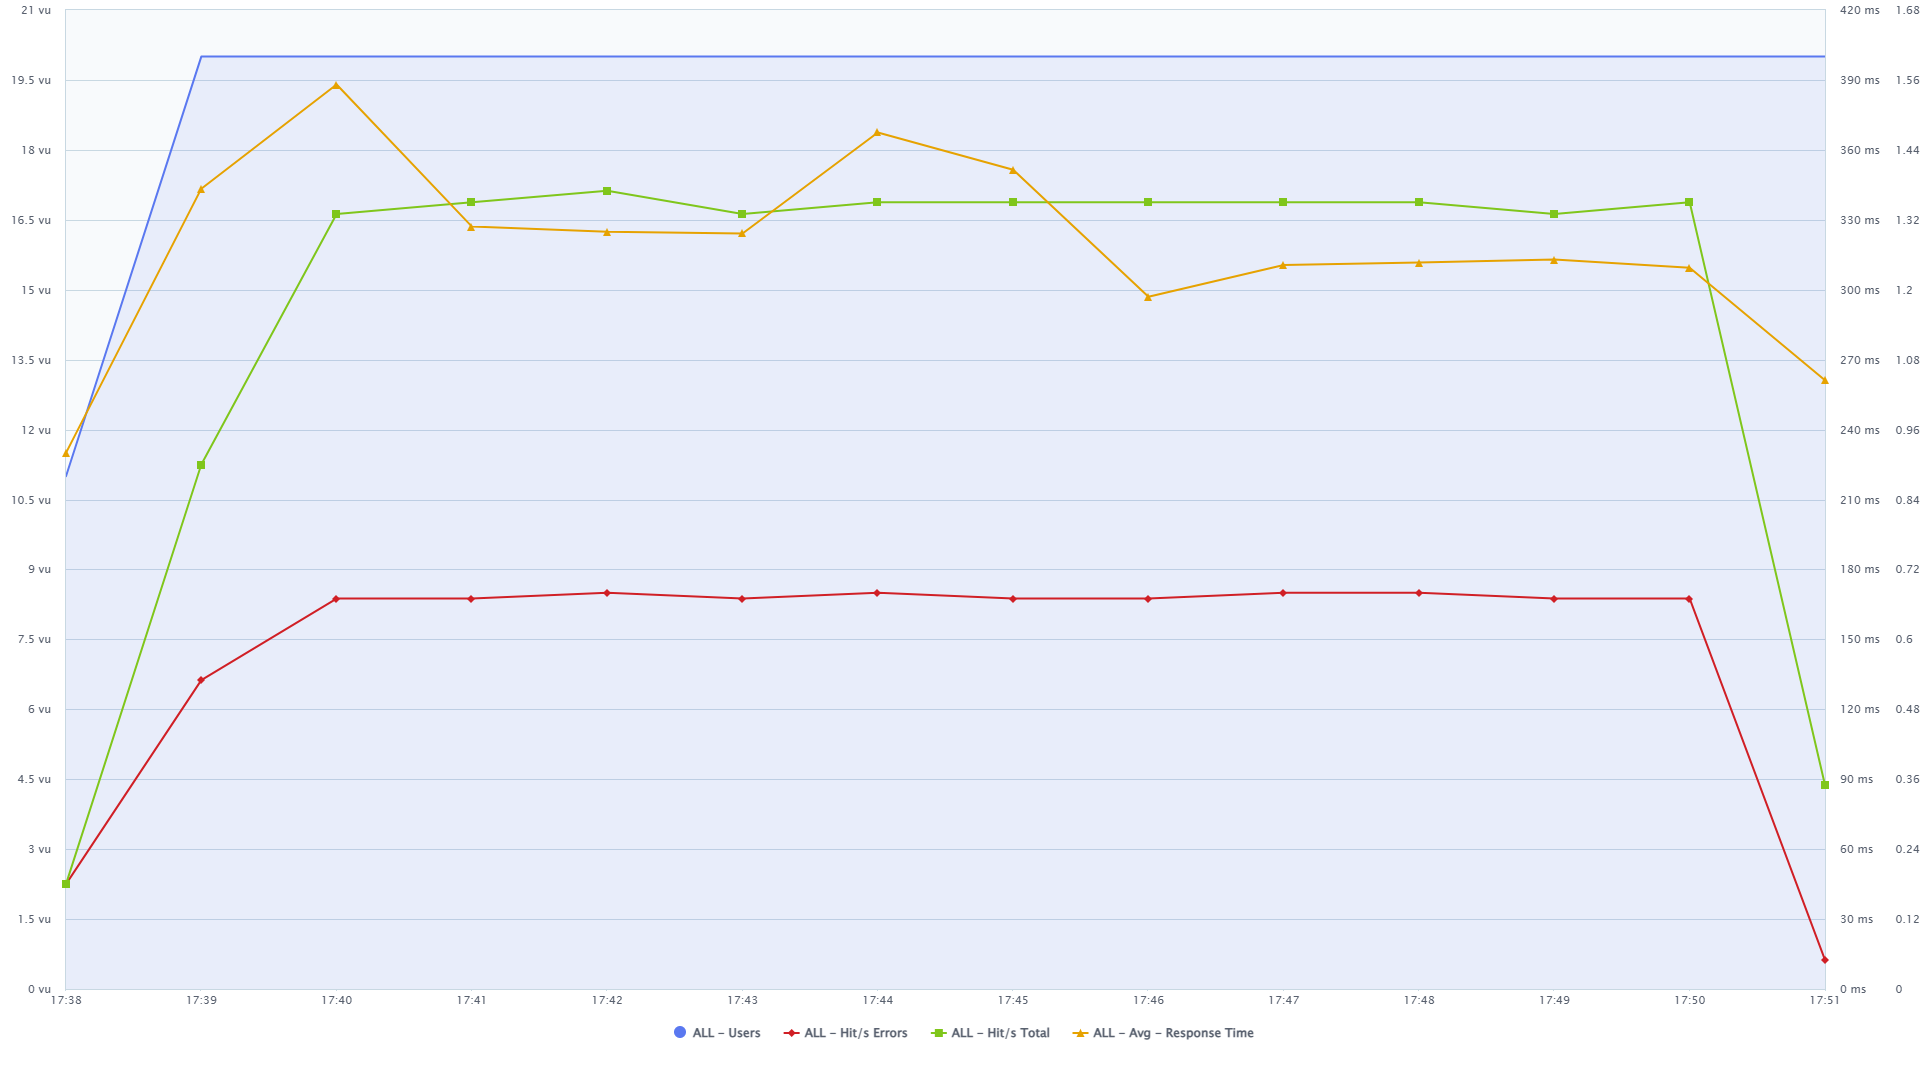
\includegraphics[width=1\textwidth]{new-chart-1-e13fd45c-e039-48c1-bb7f-3b555841f526.png}
\caption{Stress test - JMeter 20 Mock Users}
\label{fig:myimage}
\end{figure}

\newpage

For environmental-2, we leveraged Netlify's powerful development platform. Netlify facilitated the creation of a self-contained and fully functional development environment, streamlining the workflow and significantly enhancing productivity. The developers were able to set up their local environments effortlessly, following the instructions provided, and could launch the development setup with confidence, knowing it would initialize and run without errors.
\\ \\
For environmental-3, we are using GitHub issues to keep track of the dates and time for the project. Issues are created for the tasks that are remaining to be performed along with attaching the development branch that focuses on it. This way, we are able to ensure that the functional, non-functional and outside requirements are being fulfilled on-time.


\subsection{Maintenance}

\begin{center}
\begin{longtable}{|p{4cm} | p{4cm}| }
\caption{Maintenance tests}
\hline
\textbf{Test Id} & \textbf{Result} \\
\hline
maintenance-1 & Pass \\
\hline
maintenance-2 & Pass \\
\hline
maintenance-3 & Pass \\
\hline
maintenance-4 & Pass \\
\hline
maintenance-5 & Pass \\
\hline

\end{longtable}
\end{center}

\\
For maintenance-1, this system test was manually tested through the frontend. Upon executing a command, logs of a command are stored in MongoDB as JSON objects instead of plain or text files.
\\ \\
For maintenance-2, GitHub Actions is correctly configured for the project, triggering automated build and test checks. The test checks are triggered every commit, and every PR, seamlessly integrated in the Github repository.
\\ \\
For maintenance-3, the system identifies an outdated version automatically by utilizing node’s npm install command before the server is ran, and applies any changes (upgrades and downgrades). In addition, deliberate code formatting issues were introduced, and automatically corrected by esLint, the chosen code linter.
\\ \\
For maintenance-4, the project directory structure is intuitive, code is divided into client and server folders (front-end and back-end), with components, styles, and pages being divided for logical ordering. Variable, function, and template names follow consistent naming schemes, and are grouped where needed. Lastly, rigorous code reviews are performed to maintain the quality of the repository.
\\ \\
For maintenance-5, A code formatting tool, ESLint is integrated in the development environment through Visual Studio Code, and is enforced in code review. Since it is automatically integrated, random code files which are inspected match indentation, variable naming, and code structure.


\subsection{Integrity}

\begin{center}
\begin{longtable}{|p{4cm} | p{4cm}| }
\caption{Integrity Tests}
\hline
\textbf{Test Id} & \textbf{Result} \\
\hline
integrity-5 & Pass \\
\hline
integrity-6 & Pass \\
\hline
integrity-7 & Pass \\
\hline

\end{longtable}
\end{center}

For integrity-5, various simulated satellite failures have been implemented in test cases to test and monitor error messages which are consistent amongst other messages, and communicate the nature of missing data attributes.
\\ \\
For integrity-6, the application performs essential functionalities on all browsers (Safari, Chrome, Firefox).
\\ \\
For integrity-7, the typescript compiler verifies HTML and CSS validity, and has not identified any compatibility issues across devices. In addition, esLint is applied to apply HTML and CSS coding standards when it comes to formatting. The application user interface remains consistent and functional across different devices and browsers.
		
\subsection{Privacy and Accessibility}

\begin{center}
\begin{longtable}{|p{4cm} | p{4cm}| }
\caption{Privacy and Accessibility Tests}
\hline
\textbf{Test Id} & \textbf{Result} \\
\hline
access-1 & Pass \\
\hline
access-2 & Pass \\
\hline
privacy-1 & Pass \\
\hline

\end{longtable}
\end{center}

For access-1, the application integrates with an external authentication service (Auth0) to manage user authentication and account management. New and existing users will be registered and logged in using this service The test cases for this requirement are AM2 and AM3 and it can be found below in section 8 of Regression Testing.
\\ \\
For access-2, the application integrates with an external authentication service (Auth0) to manage user authentication and account management. This service allows an administrator to configure a rate limit of 10 login attempts per minute. As a result, the application enforces a 1 minute timeout period before the user can attempt to authenticate again. The test case for requirement is AM1 and it can be found below in section 8 of Regression Testing.
\\ \\
For privacy-1, the test case for this requirement has not been implemented yet. Refer to test case REG-SAT1 in section 8 of Regression Testing.

\section{Unit Testing}

\subsection{Scheduling Module}
\subsubsection{API Endpoints}


POST /schedule/createScheduledCommand


\begin{center}
\begin{longtable}{|p{1cm} | p{2cm} |p{2cm}| p{2cm} |p{2cm}| p{2cm}|}
\caption{Unit Tests for  \newline 
POST /schedule/createScheduledCommand}
\hline
\textbf{Id} & \textbf{Reference Req. Id} & \textbf{Input} & \textbf{Expected Output} & \textbf{Actual Output} & \textbf{Result} \\
\hline
SM1 & FR-12, FR-13, FR-17, FR-16  & { userId: ObjectID,
satelliteId: ObjectID,
commandId: ObjectID,
command: “start” } & { userId: ObjectID,
satelliteId: ObjectID,
commandId: ObjectID,
command: “start” } & { userId: ObjectID,
satelliteId: ObjectID,
commandId: ObjectID,
command: “start” } & Pass
\\
\hline
SM2 & FR-17, FR-16, FR-13 & { userId: ObjectID,
satelliteId: ObjectID,
commandId: ObjectID,
command: “commandNotInCriteria” }
 & { status: 500,
Error: "Invalid command sequence or user permissions" }
 & { status: 500,
Error: "Invalid command sequence or user permissions" }
 & Pass
\\
\hline

\end{longtable}

\end{center}

PATCH /schedule/updateScheduledCommand

\begin{center}
\begin{longtable}{|p{1cm} | p{2cm} |p{2cm}| p{2cm} |p{2cm}| p{2cm}|}
\caption{Unit Tests for \newline PATCH /schedule/updateScheduledCommand}
\hline
\textbf{Id} & \textbf{Reference Req. Id} & \textbf{Input} & \textbf{Expected Output} & \textbf{Actual Output} & \textbf{Result} \\
\hline
SM3 & FR-3, FR-4, FR-5 & { userId: ObjectID,
satelliteId: ObjectID,
commandId: ObjectID,
command: “start” } & { userId: ObjectID,
satelliteId: ObjectID,
commandId: ObjectID,
command: “start” } & { userId: ObjectID,
satelliteId: ObjectID,
commandId: ObjectID,
command: “start” } & Pass
\\
\hline
SM4 & FR-11 & { userId: ObjectID,
satelliteId: ObjectID,
commandId: ObjectID,
command: “commandNotInCriteria” }
 & { status: 500,
Error: "Invalid command sequence or user permissions" }
 & { status: 500,
Error: "Invalid command sequence or user permissions" }
 & Pass
\\
\hline

\end{longtable}

\end{center}

GET /schedule/getSchedulesBySatellite

\begin{center}
\begin{longtable}{|p{1cm} | p{2cm} |p{2cm}| p{2cm} |p{2cm}| p{2cm}|}
\caption{Unit Tests for \newline GET /schedule/getSchedulesBySatellite}
\hline
\textbf{Id} & \textbf{Reference Req. Id} & \textbf{Input} & \textbf{Expected Output} & \textbf{Actual Output} & \textbf{Result} \\
\hline
SM5 & FR-13 & { satelliteId: ObjectID } & { Message: “Fetched schedules”,
schedules: Schedule[] } & { Message: “Fetched schedules”,
schedules: Schedule[] } & Pass
\\
\hline
SM6 & FR-13 & { satelliteId: ObjectID,
status: “PASSED” } & { Message: “Fetched schedules”,
schedules: Schedule[] } & { Message: “Fetched schedules”,
schedules: Schedule[] } & Pass
\\
\hline

\end{longtable}

\end{center}

GET /schedule/getCommandsBySchedule


\begin{center}
\begin{longtable}{|p{1cm} | p{2cm} |p{2cm}| p{2cm} |p{2cm}| p{2cm}|}
\caption{Unit Tests for \newline GET /schedule/getCommandsBySchedule}
\hline
\textbf{Id} & \textbf{Reference Req. Id} & \textbf{Input} & \textbf{Expected Output} & \textbf{Actual Output} & \textbf{Result} \\
\hline
SM7 & FR-13 & { satelliteId: ObjectID } & { Message: “Fetched commands”,
commands: Command[] } & { Message: “Fetched commands”,
commands: Command[] } & Pass
\\
\hline

\end{longtable}

\end{center}

DELETE /schedule/deleteScheduledCommand

\begin{center}
\begin{longtable}{|p{1cm} | p{2cm} |p{2cm}| p{2cm} |p{2cm}| p{2cm}|}
\caption{Unit Tests for \newline DELETE /schedule/deleteScheduledCommand}
\hline
\textbf{Id} & \textbf{Reference Req. Id} & \textbf{Input} & \textbf{Expected Output} & \textbf{Actual Output} & \textbf{Result} \\
\hline
SM8 & FR-13 & { commandId: ObjectID,
userId: ObjectID } & { Message: “Success. Deleted schedule” } & { Message: “Success. Deleted schedule” } & Pass
\\
\hline
SM9 & FR-11 & { commandId: ObjectID,
userId: ObjectID } & { status: 500,
Error: “Insufficient permissions” } & { status: 500,
Error: “Insufficient permissions” } & Pass
\\
\hline

\end{longtable}

\end{center}

GET /satellite/getSatelliteInfo

\begin{center}
\begin{longtable}{|p{1cm} | p{2cm} |p{2cm}| p{2cm} |p{2cm}| p{2cm}|}
\caption{Unit Tests for \newline GET /satellite/getSatelliteInfo}
\hline
\textbf{Id} & \textbf{Reference Req. Id} & \textbf{Input} & \textbf{Expected Output} & \textbf{Actual Output} & \textbf{Result} \\
\hline
SM10 & FR-15 & {  } & { status: 200 } & { status: 200 } & Pass
\\
\hline
\end{longtable}

\end{center}

GET /getPolarPlotData

\begin{center}
\begin{longtable}{|p{1cm} | p{2cm} |p{2cm}| p{2cm} |p{2cm}| p{2cm}|}
\caption{Unit Tests for \newline GET /getPolarPlotData}
\hline
\textbf{Id} & \textbf{Reference Req. Id} & \textbf{Input} & \textbf{Expected Output} & \textbf{Actual Output} & \textbf{Result} \\
\hline
SM11 & FR-15 & { startTime = 2024-01- 06T 10:15:00Z;
    endTime = 2024-01- 06T 10:22:00Z;} & { status: 200 } & { status: 200 } & Pass
\\
\hline
SM12 & FR-15 & { startTime = 2024-01- 06T 10:15:00Z;
    endTime = "";} & { status: 500 } & { status: 500 } & Pass
\\
\hline

\end{longtable}

\end{center}
GET /maxElevation

\begin{center}
\begin{longtable}{|p{1cm} | p{2cm} |p{2cm}| p{2cm} |p{2cm}| p{2cm}|}
\caption{Unit Tests for \newline GET /maxElevation}
\hline
\textbf{Id} & \textbf{Reference Req. Id} & \textbf{Input} & \textbf{Expected Output} & \textbf{Actual Output} & \textbf{Result} \\
\hline
SM13 & FR-16 & { startTime = 2024-01- 06T 10:15:00Z;
    endTime = 2024-01- 06T 10:22:00Z;} & { status: 200 } & { status: 200 } & Pass
\\
\hline
SM14 & FR-16 & { startTime = 2024-01- 06T 10:15:00Z;
    endTime = "";} & { status: 500 } & { status: 500 } & Pass
\\
\hline

\end{longtable}

\end{center}
GET /getNextPasses

\begin{center}
\begin{longtable}{|p{1cm} | p{2cm} |p{2cm}| p{2cm} |p{2cm}| p{2cm}|}
\caption{Unit Tests for \newline GET /getNextPasses}
\hline
\textbf{Id} & \textbf{Reference Req. Id} & \textbf{Input} & \textbf{Expected Output} & \textbf{Actual Output} & \textbf{Result} \\
\hline
SM15 & FR-15 & { TLE = 59909 } & { status: 200 } & { status: 200 } & Pass
\\
\hline
SM16 & FR-15 & { TLE = ""} & { status: 500 } & { status: 500 } & Pass
\\
\hline

\end{longtable}

\end{center}
GET /getSolarIllumination

\begin{center}
\begin{longtable}{|p{1cm} | p{2cm} |p{2cm}| p{2cm} |p{2cm}| p{2cm}|}
\caption{Unit Tests for \newline GET /getSolarIllumination}
\hline
\textbf{Id} & \textbf{Reference Req. Id} & \textbf{Input} & \textbf{Expected Output} & \textbf{Actual Output} & \textbf{Result} \\
\hline
SM16 & FR-15 & { TLE = 59909 } & { status: 200 } & { status: 200 } & Pass
\\
\hline
SM17 & FR-15 & { TLE = ""} & { status: 500 } & { status: 500 } & Pass
\\
\hline

\end{longtable}

\end{center}

POST /changeTLE

\begin{center}
\begin{longtable}{|p{1cm} | p{2cm} |p{2cm}| p{2cm} |p{2cm}| p{2cm}|}
\caption{Unit Tests for \newline POST /changeTLE}
\hline
\textbf{Id} & \textbf{Reference Req. Id} & \textbf{Input} & \textbf{Expected Output} & \textbf{Actual Output} & \textbf{Result} \\
\hline
SM18 & FR-14 & { TLE = 59909 } & { status: 200 } & { status: 200 } & Pass
\\
\hline
SM19 & FR-14 & { TLE = ""} & { status: 500 } & { status: 500 } & Pass
\\
\hline

\end{longtable}

\end{center}

\subsection{Satellite Users Module}
\subsubsection{API Endpoints}


POST /satelliteUser/createSatelliteUser


\begin{center}
\begin{longtable}{|p{1cm} | p{3cm} |p{2cm}| p{2cm} |p{2cm}|}
\caption{Unit Tests for \newline POST /satelliteUser/createSatelliteUser}
\hline
\textbf{Id}  & \textbf{Input} & \textbf{Expected Output} & \textbf{Actual Output} & \textbf{Result} \\
\hline
SUM1 &  { userId: ObjectID,
satelliteId: ObjectID,
adminId: ObjectID,
validCommands: [“teardown”] } & { satelliteUserId: ObjectID,
satelliteId: ObjectID,
validCommands: ["teardown"],
adminId: ObjectId } & { satelliteUserId: ObjectID,
satelliteId: ObjectID,
adminId: ObjectID,
validCommands: [“teardown”] } & Pass
\\
\hline
SUM2 &  { userId: ObjectID,
satelliteId: ObjectID, adminId: "invalidAdminId",
validCommands: [“teardown”] } 
& { status: 500,
Error: "Invalid command sequence or user permissions" }
 & { status: 500,
Error: "Invalid command sequence or user permissions" }
 & Pass
\\
\hline
SUM3 &  { userId: ObjectID,
satelliteId: "invalidSatelliteId",
adminId: ObjectId,
validCommands: [“teardown”] }
 & { status: 500,
Error: "Invalid Ids" }
 & { status: 500,
Error: "Invalid Ids" }
 & Pass
\\
\hline
SUM4 &  { userId: ObjectID,
satelliteId: ObjectID,
adminId: ObjectId,
validCommands: [“invalidCommand”] }
 & { status: 500,
Error: "Invalid command sequence or user permissions" }
 & { status: 500,
Error: "Invalid command sequence or user permissions" }
 & Pass
\\
\hline
SUM5 &  { userId: "invalidUserId",
satelliteId: ObjectID,
adminId: ObjectId,
validCommands: [“teardown”] }
 & { status: 500,
Error: "Invalid command sequence or user permissions" }
 & { status: 500,
Error: "Invalid command sequence or user permissions" }
 & Pass
\\
\hline

\end{longtable}

\end{center}
PATCH /satelliteUser/updateByUser


\begin{center}
\begin{longtable}{|p{2cm} | p{3cm} |p{2cm}| p{2cm} |p{2cm}|}
\caption{Unit Tests for \newline PATCH /satelliteUser/updateByUser}
\hline
\textbf{Id}  & \textbf{Input} & \textbf{Expected Output} & \textbf{Actual Output} & \textbf{Result} \\
\hline
SUM6 &  { satelliteUserId: ObjectID,
satelliteId: ObjectID,
adminId: ObjectID,
validCommands: [“teardown”] } & { satelliteUserId: ObjectID,
satelliteId: ObjectID,
validCommands: ["teardown"],
adminId: ObjectId } & { satelliteUserId: ObjectID,
satelliteId: ObjectID,
adminId: ObjectID,
validCommands: [“teardown”] } & Pass
\\
\hline
SUM7 &  { satelliteUserId: ObjectID,
satelliteId: ObjectID,
adminId: "invalidAdminId",
validCommands: [“teardown”] }
 & { status: 500,
Error: "Invalid command sequence or user permissions" }
 & { status: 500,
Error: "Invalid command sequence or user permissions" }
 & Pass
\\
\hline
SUM8 &   { satelliteUserId: ObjectID,
satelliteId: "invalidSatelliteId",
adminId: ObjectId,
validCommands: [“teardown”] }
 & { status: 500,
Error: "Invalid Ids" }
 & { status: 500,
Error: "Invalid Ids" }
 & Pass
\\
\hline
SUM9 &   { satelliteUserId: ObjectID,
satelliteId: ObjectID,
adminId: ObjectId,
validCommands: [“invalidCommand”] }
 & { status: 500,
Error: "Invalid command sequence or user permissions" }
 & { status: 500,
Error: "Invalid command sequence or user permissions" }
 & Pass
\\
\hline
SUM10 &   { satelliteUserId: "invalidSatelliteUserId",
satelliteId: ObjectID,
adminId: ObjectId,
validCommands: [“teardown”] }
 & { status: 500,
Error: "Invalid command sequence or user permissions" }
 & { status: 500,
Error: "Invalid command sequence or user permissions" }
 & Pass
\\
\hline

\end{longtable}

\end{center}


GET /satelliteUser/getUserBySatellite

\begin{center}
\begin{longtable}{|p{2cm} | p{3cm} |p{2cm}| p{2cm} |p{2cm}|}
\caption{Unit Tests for \newline GET /satelliteUser/getUserBySatellite}
\hline
\textbf{Id}  & \textbf{Input} & \textbf{Expected Output} & \textbf{Actual Output} & \textbf{Result} \\
\hline
SUM11 &  { satelliteId: ObjectID } & { Message: “Fetched satellite users”,
satelliteUsers: satelliteUsers[] } & { Message: “Fetched satellite users”,
satelliteUsers: satelliteUsers[] } & Pass
\\
\hline
SUM12  & { satelliteId: "invalidSatelliteId"} & { Message: “Fetched satellite Users”,
satelliteUsers: [] } & { Message: “Fetched satellite Users”,
satelliteUsers: [] } & Pass
\\
\hline

\end{longtable}

\end{center}


GET /satelliteUser/getCommandsBySatelliteAndUser

\begin{center}
\begin{longtable}{|p{1.5cm} | p{3cm} |p{2cm}| p{2cm} |p{2cm}|}
\caption{Unit Tests for \newline GET /satelliteUser/getCommandsBySatelliteAndUser}
\hline
\textbf{Id} & \textbf{Input} & \textbf{Expected Output} & \textbf{Actual Output} & \textbf{Result} \\
\hline
SUM13 &   { satelliteId: ObjectID, userId: ObjectId } & { Message: “Fetched satellite users”,
satelliteUsers: satelliteUsers[] } & { Message: “Fetched satellite users”,
satelliteUsers: satelliteUsers[] } & Pass
\\
\hline
SUM14 &   { satelliteId: "invalidSatelliteId", userId: ObjectId} & { Message: “Fetched satellite Users”,
satelliteUsers: [] } & { Message: “Fetched satellite Users”,
satelliteUsers: [] } & Pass
\\
\hline
SUM15 &   { satelliteId: ObjectId, userId: "InvalidUserId"} & { Message: “Fetched satellite Users”,
satelliteUsers: [] } & { Message: “Fetched satellite Users”,
satelliteUsers: [] } & Pass
\\
\hline

\end{longtable}

\end{center}

DELETE /satelliteUser/deleteByUser

\begin{center}
\begin{longtable}{|p{1.5cm} | p{3cm} |p{2cm}| p{2cm} |p{2cm}|}
\caption{Unit Tests for \newline DELETE /satelliteUser/deleteByUser}
\hline
\textbf{Id}  & \textbf{Input} & \textbf{Expected Output} & \textbf{Actual Output} & \textbf{Result} \\
\hline
SUM16 &  { adminId: ObjectID, satelliteUserId: ObjectId } & { Message: "Removed User from satellite”} & { Message: "Removed User from satellite"} & Pass
\\
\hline
SUM17 & { adminId: "invalidAdminId", satelliteUserId: ObjectId} & { Message: "Invalid Ids"} & { Message: "Invalid Ids" } & Pass
\\
\hline
SUM18 & { satelliteUserId: "invalidId", adminId: ObjectId} & { Message: "Invalid Ids"} & { Message: "Invalid Ids" } & Pass
\\
\hline

\end{longtable}

\end{center}

\subsection{Helper Functions}

executeScheduledCommands(satelliteId: ObjectID, scheduleId: ObjectID) $\Rightarrow$ void

\begin{center}
\begin{longtable}{|p{1cm} | p{2cm} |p{2cm}| p{2cm} |p{2cm}| p{2cm}|}
\caption{Unit Tests for executeScheduledCommands()}
\hline
\textbf{Id} & \textbf{Reference Req. Id} & \textbf{Input} & \textbf{Expected Output} & \textbf{Actual Output} & \textbf{Result} \\
\hline
SM20 & FR-10 & { satelliteId: ObjectID,
scheduleId: ObjectID } & List of log records corresponding to the executed command records for the specified scheduleId & List of log records corresponding to the executed command records for the specified scheduleId & Pass
\\
\hline

\end{longtable}

\end{center}

rescheduleLeftoverCommand(satelliteId: ObjectID, scheduleId: ObjectID) $\Rightarrow$ void

\begin{center}
\begin{longtable}{|p{1cm} | p{2cm} |p{2cm}| p{2cm} |p{2cm}| p{2cm}|}
\caption{Unit Tests for rescheduleLeftoverCommand()}
\hline
\textbf{Id} & \textbf{Reference Req. Id} & \textbf{Input} & \textbf{Expected Output} & \textbf{Actual Output} & \textbf{Result} \\
\hline
SM21 & FR-10, FR-11 & { satelliteId: ObjectID,
scheduleId: ObjectID } & Schedule specified in the request has no commands with status:
 {status: “QUEUED”}
 & Schedule specified in the request has no commands with status:
 {status: “QUEUED”} & Pass
\\
\hline

\end{longtable}

\end{center}

addSchedulesForNext7Days(satelliteId: ObjectID, noradId: number) $\Rightarrow$ void

\begin{center}
\begin{longtable}{|p{1cm} | p{2cm} |p{2cm}| p{2cm} |p{2cm}| p{2cm}|}
\caption{Unit Tests for addSchedulesForNext7Days()}
\hline
\textbf{Id} & \textbf{Reference Req. Id} & \textbf{Input} & \textbf{Expected Output} & \textbf{Actual Output} & \textbf{Result} \\
\hline
SM22 & FR-16, FR-17 & { satelliteId: ObjectID,
noradId: number } & Satellite specified in the request has new schedules for the next seven days
 & Satellite specified in the request has new schedules for the next seven days & Pass
\\
\hline

\end{longtable}

\end{center}

getSatelliteInfo(date: Date, tleLine1: number, tleLine2: number) $\Rightarrow$ \{
    positionEci: number,
    velocityEci: number,
    longitude: number,
    latitude: number,
    height: number,
    azimuth: number,
    elevation: number,
    rangeSat: number
  \}

\begin{center}
\begin{longtable}{|p{1cm} | p{2cm} |p{2cm}| p{2cm} |p{2cm}| p{2cm}|}
\caption{Unit Tests for \newline getSatelliteInfo()}
\hline
\textbf{Id} & \textbf{Reference Req. Id} & \textbf{Input} & \textbf{Expected Output} & \textbf{Actual Output} & \textbf{Result} \\
\hline
SM23 & FR-15 & { new Date(), 1 55098U 23001CT  23359.66872105  .00021921  00000-0  89042-3 0  9991, 2 55098  97.4576  58.0973 0014812  57.5063 302.7604 15.24489013 54199 } & \{
    positionEci: number,
    velocityEci: number,
    longitude: number,
    latitude: number,
    height: number,
    azimuth: number,
    elevation: number,
    rangeSat: number
  \}
 & \{
    positionEci: number,
    velocityEci: number,
    longitude: number,
    latitude: number,
    height: number,
    azimuth: number,
    elevation: number,
    rangeSat: number
  \} & Pass
\\
\hline
SM24 & FR-15 & { "", 1 55098U 23001CT  23359.66872105  .00021921  00000-0  89042-3 0  9991, 2 55098  97.4576  58.0973 0014812  57.5063 302.7604 15.24489013 54199 } & Error: Invalid Date
 & Error: Invalid Date & Pass
 \\
\hline
SM25 & FR-15 & { new Date(), "", "" } & Error: Invalid TLE
 & Invalid TLE & Pass
 \\
 \hline
\end{longtable}

\end{center}

isSunLit(date: Date, lon: number,
  lat: number,
  height: number) $\Rightarrow$ boolean

\begin{center}
\begin{longtable}{|p{1cm} | p{2cm} |p{2cm}| p{2cm} |p{2cm}| p{2cm}|}
\caption{Unit Tests for isSunLit()}
\hline
\textbf{Id} & \textbf{Reference Req. Id} & \textbf{Input} & \textbf{Expected Output} & \textbf{Actual Output} & \textbf{Result} \\
\hline
SM26 & FR-15 & { new Date(), 0, 0, 0 } & isDefined
 & isDefined & Pass
\\
\hline
SM27 & FR-15 & { "", 0, 0, 0 } & isNotDefined
 & isNotDefined & Pass
 \\
\hline
SM28 & FR-15 & { new Date(), 0, 0, 20000} & Error: Height must be in km
 & Error: Height must be in km & Pass
 \\
 \hline
\end{longtable}

\end{center}

setTLE(tle: string) $\Rightarrow$ void

\begin{center}
\begin{longtable}{|p{1cm} | p{2cm} |p{2cm}| p{2cm} |p{2cm}| p{2cm}|}
\caption{Unit Tests for setTLE()}
\hline
\textbf{Id} & \textbf{Reference Req. Id} & \textbf{Input} & \textbf{Expected Output} & \textbf{Actual Output} & \textbf{Result} \\
\hline
SM29 & FR-14 & { "55098" } & resolves
 & resolves & Pass
\\
\hline
SM30 & FR-14 & { "abcd" } & Error: Invalid TLE
 & Error: Invalid TLE & Pass
 \\
\hline
SM31 & FR-14 & { "" } & Error: Empty TLE
 & Error: Empty TLE & Pass
 \\
 \hline
\end{longtable}

\end{center}


\section{Regression Testing}

\subsection{Authentication Module}

\begin{center}
\begin{longtable}{|p{1cm} | p{2cm} |p{2cm}| p{2cm} |p{2cm}| p{2cm}|}
\caption{Regression Tests for Authentication Module}
\hline
\textbf{Id} & \textbf{Reference Req. Id} & \textbf{Input} & \textbf{Expected Output} & \textbf{Actual Output} & \textbf{Result} \\
\hline
AM1 & NFR 14.1.2 & {email: “test1@ gmail.com”
password: “correct” } Repeat 10 times
 & Disable login functionality for one minute
 & Disable login functionality for one minute & Pass
\\
\hline
AM2 & NFR 14.1.1 & { email: "test1@ gmail.com"
password: “correct” }
 & Successfully log user into the application’s home page
 & Successfully log user into the application’s home page & Pass
\\
\hline
AM3 & NFR 14.1.1, NFR 14.1.2 & { email: “test1@ gmail.com”
password: “correct” }
 & Successfully register user into the application and directs them to the home page
 & Successfully register user into the application and directs them to the home page & Pass
\\
\hline

\end{longtable}

\end{center}

\subsection{Satellite Module}
\begin{center}
\begin{longtable}{|p{1cm} | p{2cm} |p{2cm}| p{2cm} |p{2cm}| p{2cm}|}
\caption{Regression Tests for Satellite Module}
\hline
\textbf{Id} & \textbf{Reference Req. Id} & \textbf{Input} & \textbf{Expected Output} & \textbf{Actual Output} & \textbf{Result} \\
\hline
REG-SAT1 & NFR 14.3.1 & { port: number }
 & Socket successfully connected with hash output
 & Socket successfully connected with hash output & TBD
\\
\hline

\end{longtable}

\end{center}



\section{Changes Due to Testing}

\subsection{Feedback from Revision 0}

During the Revision 0 demonstration, the application was assessed on its functionality and overall usability. The major feedback received was the lack of integration between the different functional components. For example, both user interfaces and endpoints were created to add and update valid commands, however these two components were not integrated together. This has been resolved by integrating the frontend and backend components relating to managing satellite information and valid commands for an operator. As a result, users are able to interact with the application without intervention from a developer.

\subsection{Feedback from Usability Testing}

Two usability tests have been conducted to assess the application. Each test involved stakeholders as well as new users from McMaster's NEUDOSE team to evaluate the core functionalities of the web application. 
\\ \\
From the first usability testing demonstration, the critiques mainly highlighted issues with the UI/UX of application rather than the functionality. Specifically, users mentioned that the presentation of information for upcoming satellite overpasses felt cluttered and suggested to separate information related to satellite into different sections. After reviewing the feedback from this usability test, changes to the user interface was made such that overpasses for a satellite was presented in a tabular format as opposed to a card. This improved the readability and organization of data in the frontend.
\\ \\ 
Furthermore, heading into the second usability testing demonstration with member of the NEUDOSE team, all usability issues described above had been addressed. During this demonstration, users responded positively to the new UI/UX changes, however, there were some issues when loading changes to satellite information in the frontend. This has been resolved by refactoring how the information from the backend is captured in the frontend. To address this, an external query management package known as TanStack Query was integrated into the frontend facing application to manage requests sent to the backend. This provided the ability to automatically react and load data from the backend, ensuring data changes are timely displayed. Additionally, users felt that as the number of schedules for a satellite increases, it would be difficult to find a particular schedule. This was addressed by adding a date filter for satellite passes, which enables users to search for schedules by specifying the start and end dates.

\subsection{Additional Application Changes}
Although FR-SLN2 was verified locally, the initial deployment of the application's backend did not support evaluating this test in production. When testing FR-SLN2 on the deployed backend of the application, there were issues establishing a TCP connection. For some context, the backend application was deployed using DigitalOcean's App Platform which is a containerized service. After investigating, this deployment had very limited customizing features. In particular, DigitalOcean's App Platform did not offer the ability to open a port to establish a TCP connection. As a result, a connection could not be made with the deployment build and FR-SLN2 was verified not able to be tested in production. In order to resolve this, a virtual machine (VM) had been provisioned on DigitalOcean. This VM was then configured to run the backend application. Since a VM has customizable options, a TCP port was configured which was then used to establish a valid TCP connection. Finally, the FR-SLN2 functional requirement test was verified with this new deployment.

\subsection{Changes to the VnV Plan}

FR-SLN15
\begin{itemize}
\item This test has been removed as the stakeholders no longer requested this requirement.
\end{itemize}
\\
performance-3 (NFR 11.3)
\begin{itemize}
\item Precision calculation will be tested by external library providers as the calculations are no longer in the scope of the application.
\end{itemize}
\\
access-1 (NFR 14.1.1)
\begin{itemize}
\item NFR 14.1.1 has been revised and the application will only require to support Single-Sign-On (SSO) authentication instead of Multi-Factor-Authentication (MFA).
\end{itemize}


\section{Automated Testing}

For the frontend repository, leo-client-app, we use Next.js and Netlify's built-in testing mechanism to ensure both local and production environments are error-free. Locally, developers can run the command \textbf{npm run build} to create a build directory with a production build of the application. Developers can run this command to verify that their code has no production issues before pushing from their remote machine. The execution of this command is also automated via Github Actions anytime a commit is pushed into the repository as well as during merging from feature branches to the \textbf{main} branch of the repository. Since the main branch reflects the production environment, this build check must pass before a feature branch can be merged into the main branch. In addition, a Netlify build is created through Github Actions for every feature branch being merged into the main branch. Since Netlify is hosting the frontend-facing components of the application, this build must be successful before merging into the main branch.
\\ \\
For the backend repository, leo-server-app, tests are automated using Jest.js. All unit tests pertaining to the Satellite, Schedule, and Command modules are found in the src/tests folder. Through Github Actions, all tests are automatically executed when issuing a pull request to merge to the main branch. Developers can also automate this test by running the command, \textbf{npm run test} locally. This is also the same command Github Actions uses upon pushing a commit to a branch.
		
\section{Trace to Requirements}
\begin{longtable}{|p{0.45\linewidth}|p{0.45\linewidth}|}
\hline
\textbf{Req. ID} & \textbf{System Test ID} \\
\hline
FR-1 & FR-SLN1, SM3 \\
\hline
FR-2 & FR-SLN2, FR-SLN3, FR-SLN4 \\
\hline
FR-3 & FR-SLN5, FR-SLN6 \\
\hline
FR-4 & FR-SLN5, FR-SLN6, SM3 \\
\hline
FR-5 & FR-SLN5, FR-SLN6, SM3 \\
\hline
FR-6 & FR-SLN7 \\
\hline
FR-7 & FR-SLN3, FR-SLN4, FR-SLN8 \\
\hline
FR-8 & FR-SLN8 \\
\hline
FR-10 & FR-SLN9, SM10, SM20, SM21 \\
\hline
FR-11 & FR-SLN9, SM4, SM9, SM11, SM21 \\
\hline
FR-12 & FR-SLN11, SM1 \\
\hline
FR-13 & FR-SLN12, SM5, SM6, SM7, SM8 \\
\hline
FR-14 & FR-SLN13, SM7, SM8, SM18, SM19, SM29, SM30, SM31 \\
\hline
FR-15 & FR-SLN14, SM7, SM8, SM10, SM11, SM12, SM23, SM24, SM25, SM26, SM27, SM28 \\
\hline
FR-16 & SM1, SM2, SM12, SM13, SM14, SM22 \\
\hline
FR-17 & FR-SLN16, SM1, SM2, SM12, SM22 \\
\hline
NFR-10.1 & usability-1 \\
\hline
NFR-10.3 & usability-2 \\
\hline
NFR-10.5 & usability-3 \\
\hline
NFR-11.2 & performance-2 \\
\hline
NFR-11.4 & performance-4 \\
\hline
NFR-12.2.1 & environmental-1 \\
\hline
NFR-12.2.2 & environmental-2 \\
\hline
NFR-12.5 & environmental-3 \\
\hline
NFR-13.1.1 & maintenance-1 \\
\hline
NFR-13.1.2 & maintenance-2 \\
\hline
NFR-13.1.3 & maintenance-3 \\
\hline
NFR-13.1.4 & maintenance-4 \\
\hline
NFR-13.1.5 & maintenance-5 \\
\hline
NFR-13.2.1 & support-1 \\
\hline
NFR-13.2.2 & support-2 \\
\hline
NFR-13.2.3 & support-3 \\
\hline
NFR-14.1.1 & access-1, AM2, AM3 \\
\hline
NFR-14.1.2 & access-2, AM1, AM3 \\
\hline
NFR-14.2.5 & integrity-5 \\
\hline
NFR-14.2.6 & integrity-6 \\
\hline
NFR-14.2.7 & integrity-7 \\
\hline
NFR-14.3.1 & privacy-1, REG-
SAT1 \\
\hline
\end{longtable}


\section{Trace to Modules}	

\begin{longtable}{|p{0.45\linewidth}|p{0.45\linewidth}|}
\hline
\textbf{Module} & \textbf{System Test ID} \\
\hline
Authentication Module & AM1, AM2, AM3 \\
\hline
Schedule Module & SM1, SM2, SM3, SM4, SM5, SM6, SM7, SM8, SM9, SM10, SM11, SM12 \\
\hline
Satellite User Module & SUM1, SUM2, SUM3, SUM4, SUM5, SUM6, SUM7, SUM8, SUM9, SUM10, SUM11, SUM12, SUM13, SUM14, SUM15, SUM16, SUM17, SUM18
\hline
Satellite Module & REG-SAT1 \\
\hline
\end{longtable}
\newpage
\section{Code Coverage Metrics}

The below image details the code coverage for the leo-server-app repository. This provides metrics on the percentage of statements, branches, functions, and lines covered for each file.

\begin{figure}[h]

\graphicspath{./BackendCodeCoverage/}
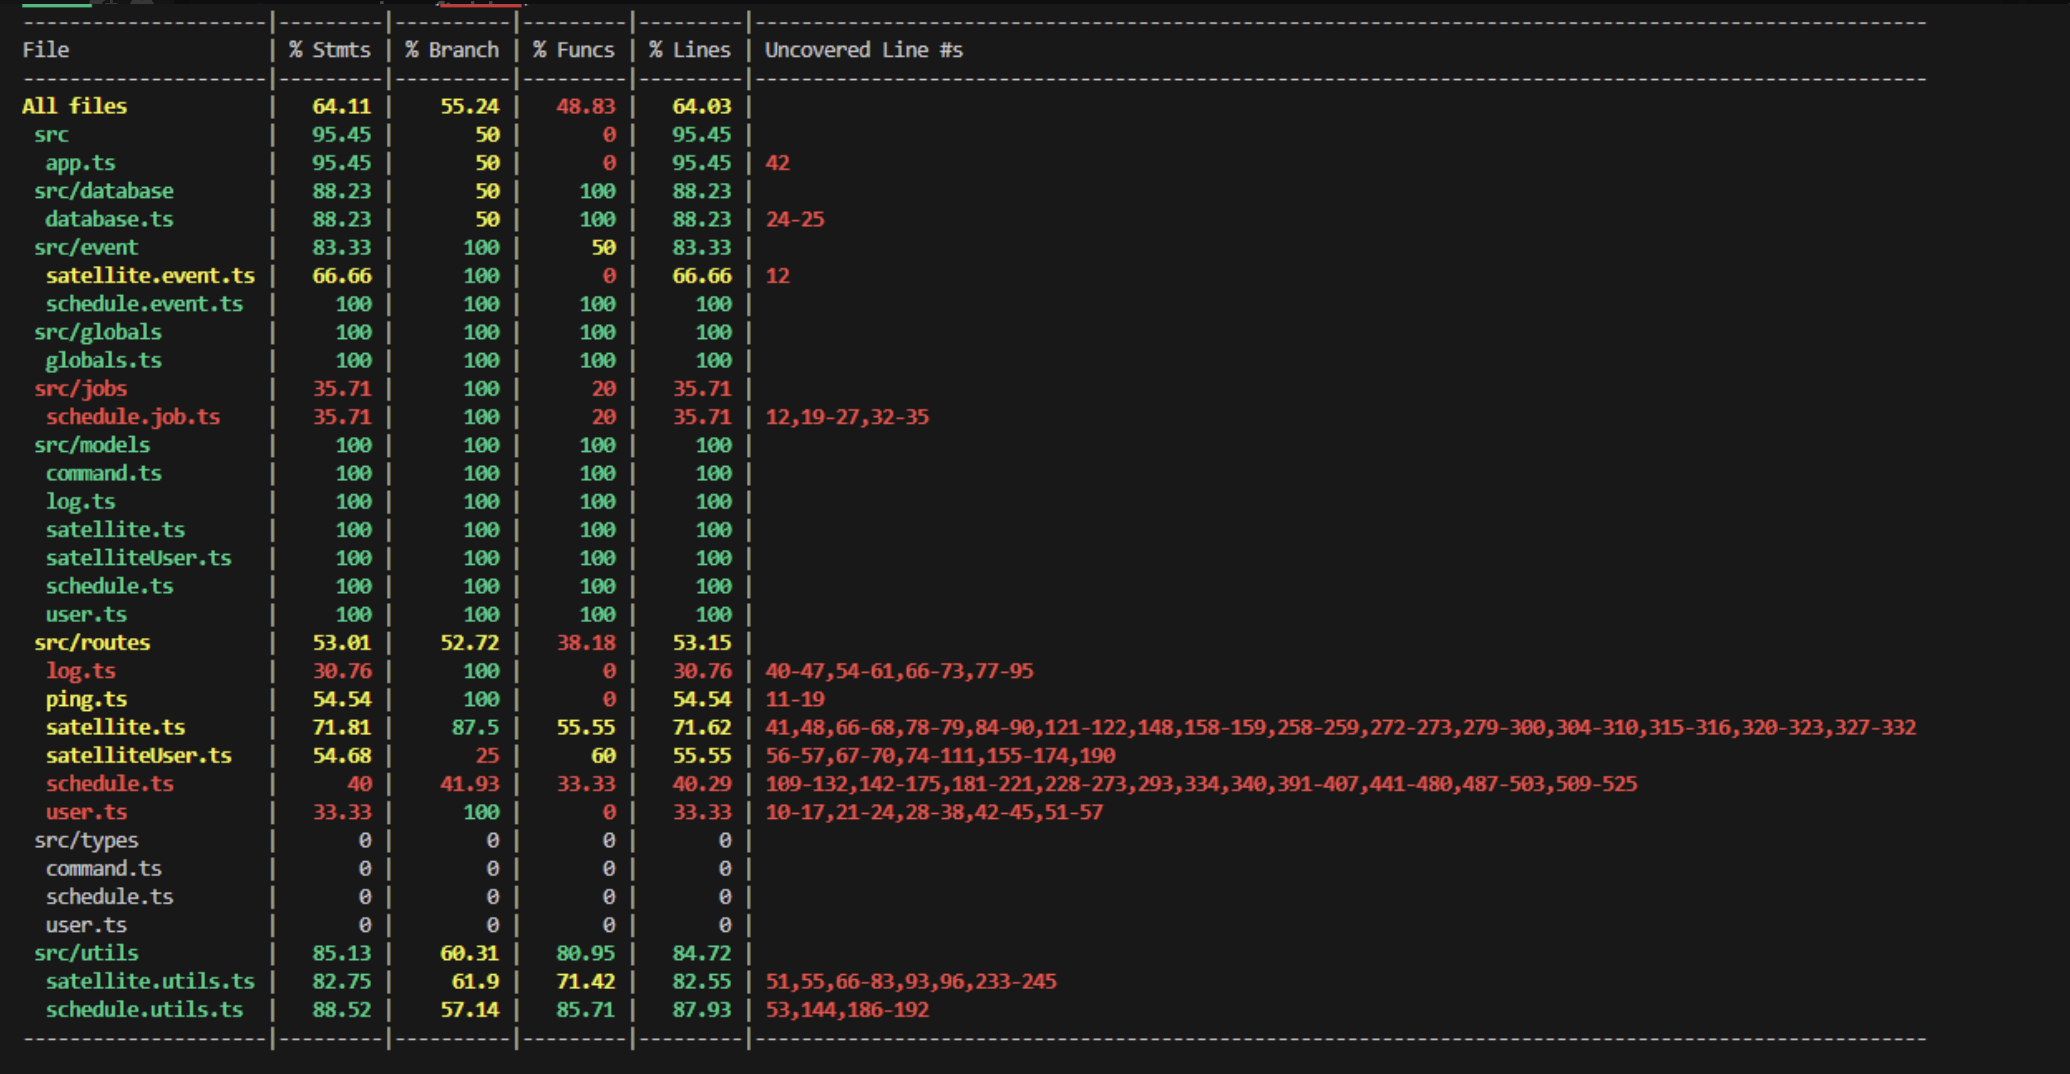
\includegraphics[width=15cm, height=10cm]
{BackendCodeCoverage.png}
\caption{Code Coverage Metrics}
\end{figure}

\section{Appendix --- Survey}
\subsection{Usability Survey Questions and Answers}

Was the application intuitive for you to use? Rate from 1-5 from least to most intuitive.

\begin{itemize}
    \item Usability Test 1: 3/5
    \item Usability Test 2: 5/5
\end{itemize}

\\ \\

Was any aspect of the application difficult to use? Provide any examples if you can. 

\begin{itemize}
    \item it's unclear how the scheduler works (i.e. you select a satellite then select a pass, then you can set commands but it's not obvious those commands have been succesfully assigned to that pass). It would be nice to be able to, from within the scheduling editor page, change which pass the schedule is being set up for.
    \item it would also be nice if once a set of commands is input for a pass the application gave some confirmation the schedule has been set and when it is set for.
    \item Not really, I thought everything was intuitive and easily navigable.
\end{itemize}

\\ \\

Did you encounter any bugs/errors/issues while you were using the application? Provide any examples if you can.

\begin{itemize}
    \item i was only there for ~10 minutes but nothing seemed to break. Not sure if setting the edit schedule with a new command (such as teardown) does anything yet, but if it's supposed to adjust the schedule the pass schedule does not seem to update with the new command
    \item The scheme could use some fixing (light\dark mode).
\end{itemize}

\\ \\

How clear and understandable was the content within the application? Were there any parts that confused you?

\begin{itemize}
    \item Interface mostly makes sense! see previous comment on scheduling being unclear when the new schedule is set
    \item I think everything was clear and easily navigable.
\end{itemize}

\\ \\

Please provide your thoughts on the overall visual design of our application. 

\begin{itemize}
    \item Generally good, the white text on light background is somewhat hard to read (sattelites, schedule, logs, etc.)
    \item I think it looked nice, simple and easy to navigate. However, the area where it displayed the satellites command schedule felt a little too cluttered.
\end{itemize}

\\ \\

Are there any aspects of the UI that you found unappealing? Please explain why.

\begin{itemize}
    \item The area where there it listed the next command schedule for satellites could benefit from a scroll bar.
\end{itemize}

\\ \\

How satisfied are you with the overall application? From a scale of 1-5 from least satisfied to most.

\begin{itemize}
    \item First test: 3/5
    \item Second test: 4/5
\end{itemize}

\\ \\

What do you like most about the application? What do you like least?

\begin{itemize}
    \item I liked how you show the schedule commands for the given week, etc. I also liked the extra information displayed for every satellite.
\end{itemize}

\\ \\

Are there any features/aspects of the application that you found useful or unnecessary? Please provide some examples. 

\begin{itemize}
    \item I think everything was very nice and nothing was redundant.
\end{itemize}

\\ \\

What part of the application in your opinion needs the most improvement. Why?

\begin{itemize}
    \item The area where it displayed the scheduled commands is the biggest issue.
\end{itemize}

\\ \\

How can we improve the application to better meet your expectations? 

\begin{itemize}
    \item More organized (possibly add tabs?) and add scroll bar.
\end{itemize}

\\ \\

Is anything missing in your opinion? What would you add? 

\begin{itemize}
    \item Scroll bar for the commands and possibly make it less cluttered, a back button would be nice. Overall good job.
\end{itemize}

\subsection{Usability Survey Notes and Summary}
\begin{itemize}
    \item The initial testing involved users with no prior experience with the application, focusing on their ability to learn and navigate the system independently. The feedback highlights both strengths and areas for enhancement in the application's design and functionality.
    \item Strengths Noted:
    \begin{itemize}
        \item The satellite and overpass functionality received positive remarks for its quick response when navigating to specific longitudes and latitudes, indicating efficient performance in these areas.
        \item The command deletion process within the application was described as "pretty solid," suggesting it is user-friendly and reliable.
    \end{itemize}
    \item Areas for Improvement:
    \begin{itemize}
        \item Visibility and Clarity: There was confusion about the "valid commands box," suggesting a need for increased visibility and clearer indications of its purpose. It's essential to make it more obvious to users what the valid commands are.
        \item Logs Page Functionality: Questions were raised about the purpose of the logs page, with suggestions to include filters for better usability, indicating a need for clearer presentation and functionality.
        \item User Interface (UI) Considerations:
        \begin{itemize}
            \item The all-white interface led to suggestions for a light mode/dark mode feature, catering to different user preferences.
            \item The addition of a feature to easily add satellites to the database directly from the first page was recommended.
            \item Faster loading times for satellite changes were requested to enhance user experience.
            \item Improvements in readability and presentation of information for upcoming satellite passes, possibly through a tabular format, were suggested to make the data more accessible.
            \item A reevaluation of navigation within the schedule queue, seeking alternatives to horizontal scrolling, was advised.
            \item The introduction of a filter for satellite passes, enabling searches by date or specific passes, was recommended to improve usability.
            \item A call for a design that avoids the need for page scrolling, aiming to present all relevant information simultaneously.
            \item The presentation of information in blocks or separated formats was suggested to improve visual hierarchy and readability, particularly for satellite information.
        \end{itemize}
    \end{itemize}
\end{itemize}






\bibliographystyle{plainnat}
\bibliography{../../refs/References}

\newpage{}
\section*{Appendix --- Reflection}

The information in this section will be used to evaluate the team members on the
graduate attribute of Reflection.  Please answer the following question:

\begin{enumerate}
  \item In what ways was the Verification and Validation (VnV) Plan different
  from the activities that were actually conducted for VnV?  If there were
  differences, what changes required the modification in the plan?  Why did
  these changes occur?  Would you be able to anticipate these changes in future
  projects?  If there weren't any differences, how was your team able to clearly
  predict a feasible amount of effort and the right tasks needed to build the
  evidence that demonstrates the required quality?  (It is expected that most
  teams will have had to deviate from their original VnV Plan.)
\end{enumerate}

\begin{itemize}
    \item Quinn - The biggest difference in the way that the VnV plan was different from what was conducted was for me, the satellite calculations. the initial plan was to develop the code to calculate, however upon future research, was determined to be more accurate to rely on scientists and utilize open-source libraries instead. As a result, the VnV plan was modified to instead validate the flow of data, specifically the data and types of the parameters. This could have been anticipated earlier with given research, and more effort will be given in the future by researching before establishing a plan for testing.
    \item Umang - In terms of verifying and validating the functionality of the scheduling and authentication modules, we initially had wanted to automate both backend and frontend facing features using a unit-testing library. However, we instead decided to modularize the evaluation of the backend and frontend components. As a result, we opted for evaluating the backend API endpoints and helper functions using unit tests to measure the application's correctness. Then, we used acceptance testing with our stakeholders to assess the user interface of the application. Furthermore, this could have been anticipated by researching into common methods of testing server and client-side applications beforehand.
    \item Diamond - Reflecting on our initial Verification and Validation (VnV) Plan, we realized the necessity to deviate from certain aspects, notably the Usability-3, NFR: 10.5, focused on assessing accessibility. This part of the plan, aimed at manually testing the application's accessibility for users with diverse needs, was ambitious in ensuring our system was universally accessible. However, due to constraints in resources, time, and the availability of a varied group of test participants with specific accessibility needs, we have decided not to proceed with this detailed testing approach. Instead, our efforts have pivoted towards leveraging best practices in accessibility design and relying on automated tools to assess some accessibility features. This decision underlines the often complex balance between ideal testing scenarios and the practical limitations of project environments. It also highlights the importance of flexibility in project management and the need to adapt plans based on available resources and evolving project dynamics. This experience reinforces the value of incorporating adaptability into our VnV strategies, allowing us to better anticipate and accommodate changes in future projects while still aiming to deliver high-quality, accessible software within our constraints.
    \item Rishi - When we look back at our initial plan for Verification and Validation (VnV) and compare it to what we actually ended up doing, we noticed quite a few differences. These changes were necessary because we encountered unexpected requirements and had to make practical adjustments to fit the scope and methods of our project. For example, we had to tweak our strategies to fit new tools and technologies, adjust to changes in our team's skills, and cope with shifts in project deadlines.
   

These adjustments were all part of the unpredictable nature of software development. Plans that look good on paper often have to be adapted to deal with the real-world challenges we face, like technical hurdles, limited resources, and changes in project goals. Going through this process taught us the importance of being flexible and able to change direction when needed. While it's hard to predict every twist and turn, this project showed us that being adaptable is key to success.

We learned that having a solid plan is essential, but so is being ready to adjust that plan as we go along and learn new things. This mindset will help us anticipate and handle changes better in future projects, making sure our VnV activities stay on track with what we're trying to achieve and the limitations we face.
 \item Dhruv - The biggest difference in our initial plan and what ended up happening was the new changes and requirements that were added along the way. As a result, practical changes are a consequence especially if we want to fit it within our timeline and scope of our project. This is only natural in software development and was an important lesson to learn because no one can ever predict all incoming changes that will happen. This forced me to not get fixated on one solution and to keep thinking from different perspectives. Additionally, we were able to do user testing with our stakeholders which provided important and useful feedback. This motivated us to research more software testing methods, even the unconventional ones perhaps. As someone who was primarily working on the front-end, I never estimated that it would take as long as it did. It was an important lesson that every aspect of software development is vital. 
\end{itemize}

\end{document}